\section{Factorizing Convolutions with Large Filter Size}

Much of the original gains of the  GoogLeNet network~\cite{szegedy2015going}
arise from a very generous use of dimension reduction. This can be viewed
as a special case of factorizing convolutions in a computationally efficient
manner. Consider for example the case of a $1\times 1$ convolutional layer
followed by a $3\times 3$ convolutional layer.
In a vision network, it is expected that the outputs
of near-by activations are highly correlated. Therefore,
we can expect that their activations can be reduced before
aggregation and that this should result in
similarly expressive local representations.

Here we explore other
ways of factorizing convolutions in various settings, especially in order to
increase the computational efficiency of the solution. Since Inception networks
are fully convolutional, each weight corresponds to one multiplication per
activation. Therefore, any reduction in computational cost results in reduced
number of parameters. This means that with suitable factorization, we can end up
with more disentangled parameters and therefore with faster training.
Also, we can use the computational and memory savings to increase the
filter-bank sizes of our network while maintaining our ability to train
each model replica on a single computer.

\subsection{Factorization into smaller convolutions}
\label{factorizing}
Convolutions with larger spatial filters (e.g. $5\times 5$ or
$7\times 7$) tend to be disproportionally expensive in terms of computation.
For example, a $5\times 5$ convolution
with $n$ filters over a grid with $m$ filters is 25/9 ~= 2.78 times
more computationally expensive
than a $3\times 3$ convolution with the same number of filters. Of course, a
$5\times 5$
filter can capture dependencies between signals between activations of units
further away in the earlier layers, so a reduction of the geometric size of the
filters comes at a large cost of expressiveness. However,
we can ask whether a $5\times 5$ convolution could be
replaced by a multi-layer network with less parameters with the same input
size and output depth. If we zoom into the computation graph of the
$5\times 5$ convolution, we see that each output looks like a small
fully-connected network sliding over $5\times 5$ tiles over its input
(see Figure~\ref{fig:double3}).
\begin{figure}
\centering
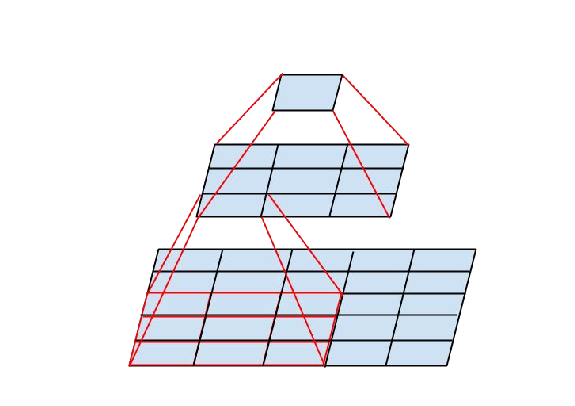
\includegraphics[width=\linewidth]{double3x3}
\caption{Mini-network replacing the $5\times 5$ convolutions.}
\label{fig:double3}
\end{figure}
Since we are constructing a vision network, it seems natural to
exploit translation invariance again and replace the fully connected component
by a two layer convolutional architecture: the first layer is a $3\times 3$
convolution, the second is a fully connected layer on top of the $3\times 3$
output grid of the first layer (see Figure~\ref{fig:double3}).
Sliding this small network over the input activation grid boils down to
replacing the $5\times 5$ convolution with two layers of $3\times 3$
convolution (compare Figure~\ref{fig:inceptionv1} with \ref{fig:inceptionv2}).

This setup clearly reduces the parameter count
by sharing the weights between adjacent tiles.
To analyze the expected computational cost savings,
we will make a few simplifying assumptions that apply for the typical
situations: We can assume that $n=\alpha m$, that is that we want to change the
number of activations/unit by a constant alpha factor. Since the $5\times 5$
convolution is aggregating, $\alpha$ is typically slightly larger
than one (around 1.5 in the case of GoogLeNet). Having a two layer replacement
for the $5\times 5$ layer, it seems reasonable to reach this expansion in two
steps: increasing the number of filters by $\sqrt{\alpha}$ in both steps.
In order to simplify our estimate by choosing $\alpha=1$ (no expansion),
If we would naivly slide a network without reusing the computation between
neighboring grid tiles, we would increase the computational cost.
sliding this network can be represented by two $3\times 3$ convolutional layers
which reuses the activations between adjacent tiles.
This way, we end up with a net $\frac{9+9}{25}\times$ reduction
of computation, resulting in a relative gain of $28\%$ by this factorization.
The exact same saving holds for the parameter count as each parameter
is used exactly once in the computation of the activation of each unit.
Still, this setup raises two general questions: Does this replacement result in
any loss of expressiveness? If our main goal is to factorize the linear part of
the computation, would it not suggest to keep linear activations in
the first layer? We have ran several control experiments
(for example see figure~\ref{fig:factorization_comparison}) and using
linear activation was always inferior to using rectified linear units in
all stages of the factorization.
We attribute this gain to the enhanced space of variations that the network
can learn especially if we batch-normalize~\cite{ioffe2015batch} the
output activations. One can see similar effects when using linear activations
for the dimension reduction components.
\begin{figure}
\centering
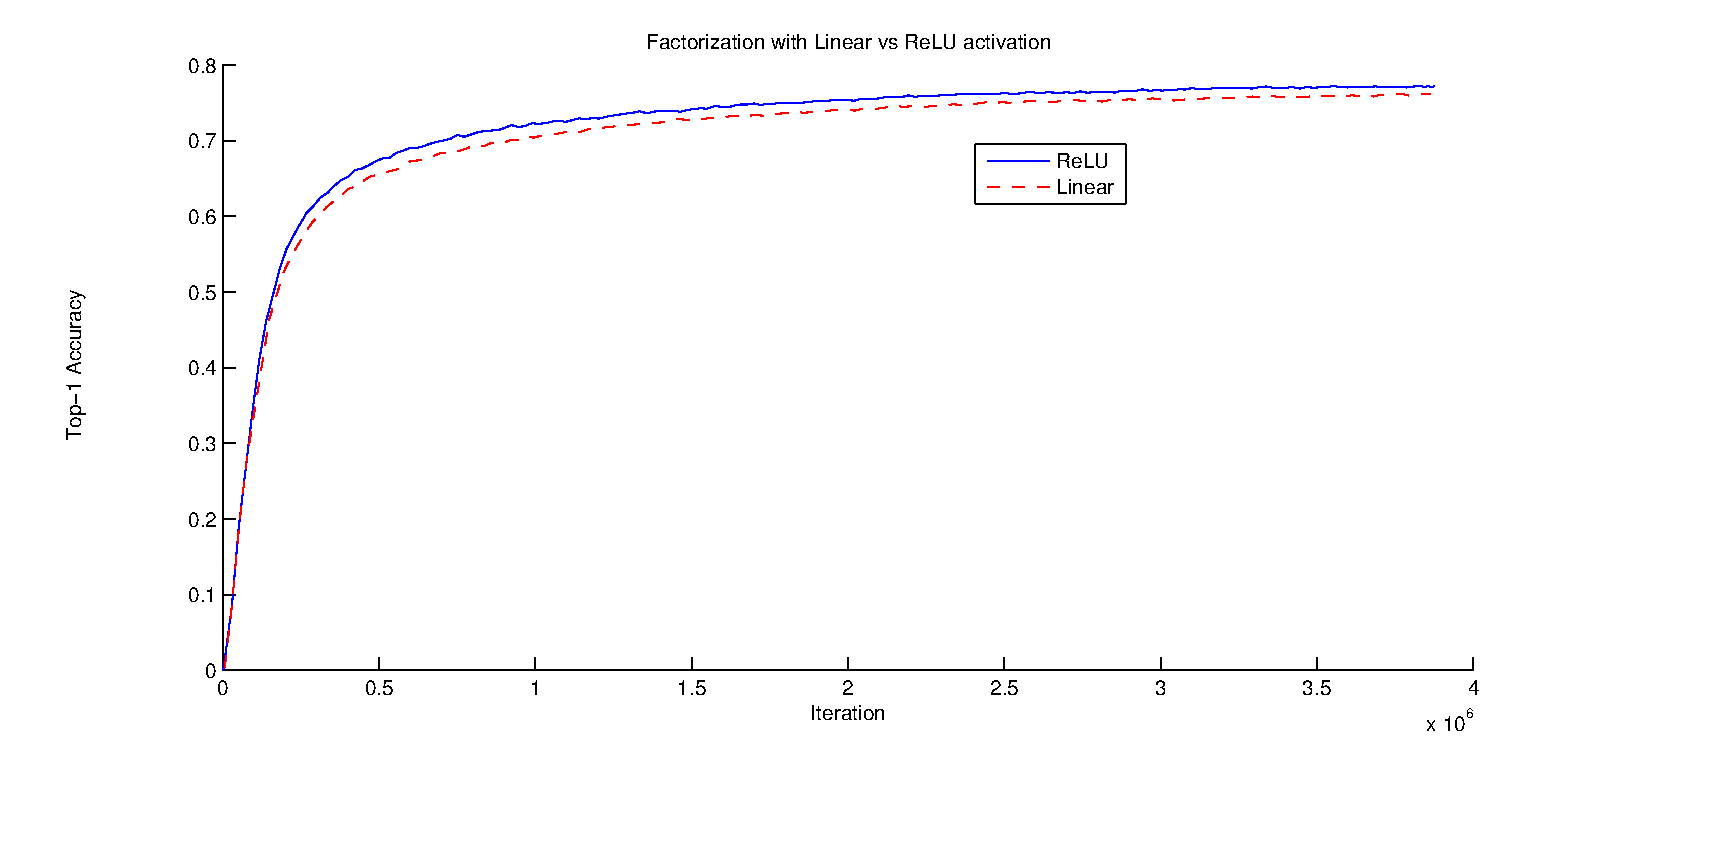
\includegraphics[width=\linewidth]{factorization_comparison}
\caption{One of several control experiments between two Inception models,
  one of them uses factorization into linear + ReLU layers, the other uses
  two ReLU layers. After $3.86$ million operations, the former settles at
  $76.2\%$, while the latter reaches $77.2\%$ top-1 Accuracy on the
  validation set.}
\label{fig:factorization_comparison}
\end{figure}

\subsection{Spatial Factorization into Asymmetric Convolutions}
The above results suggest that convolutions with filters larger
$3\times 3$  a might
not be generally useful as they can always be reduced into a sequence of
$3\times 3$ convolutional layers.
Still we can ask the question whether one should factorize them into smaller,
for example $2\times 2$ convolutions.
However, it turns out that one can do even better than $2\times 2$
by using asymmetric convolutions, e.g. $n\times 1$.
For example using a $3\times 1$ convolution followed by a $1\times 3$
convolution is equivalent to sliding a two layer network with the same
receptive field as in a $3\times 3$ convolution (see figure~\ref{fig:double31}).
Still the two-layer solution is $33\%$ cheaper for the same number of
output filters, if the number of input and output filters is equal.
\begin{figure}
\centering
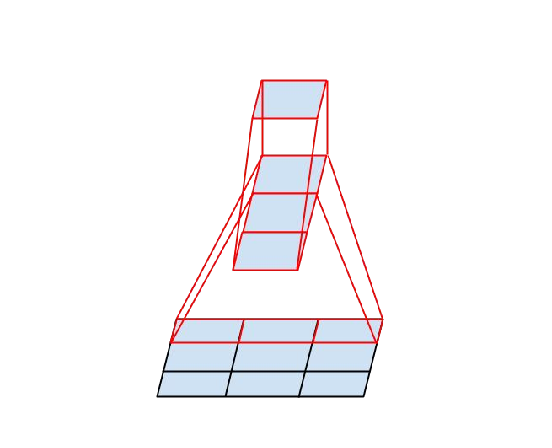
\includegraphics[width=\linewidth]{double31}
\caption{Mini-network replacing the $3\times 3$ convolutions.
  The lower layer of this network consists of a $3\times 1$ convolution with
  $3$ output units.}
\label{fig:double31}
\end{figure}
By comparison, factorizing a $3\times 3$
convolution into a two $2\times 2$ convolution represents only a $11\%$ saving
of computation.
\begin{figure}
\centering
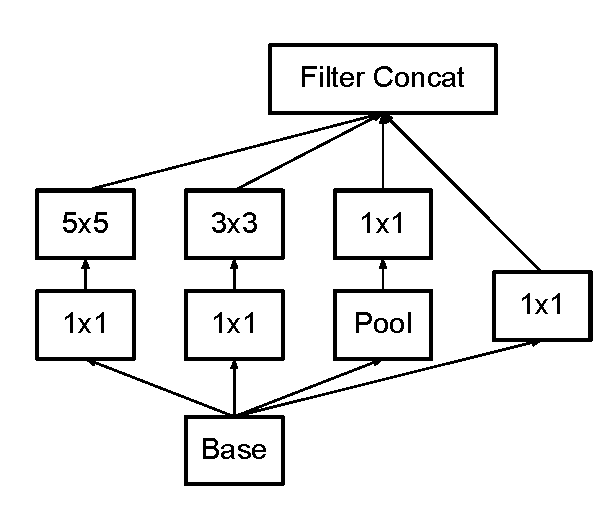
\includegraphics[width=\linewidth]{inceptionv1}
\caption{Original Inception module as described in~\cite{szegedy2015going}.}
\label{fig:inceptionv1}
\end{figure}
\begin{figure}
\centering
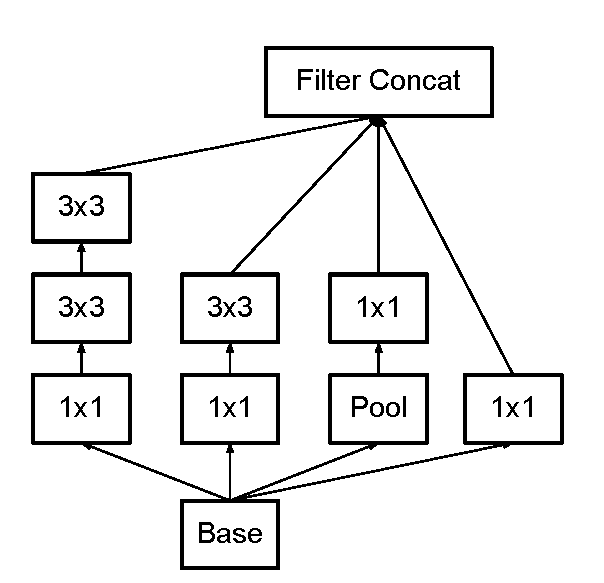
\includegraphics[width=\linewidth]{inceptionv2}
\caption{Inception modules where each $5\times 5$ convolution is replaced by
  two $3\times 3$ convolution, as suggested by principle~\ref{lowdim} of Section~\ref{principles}.}
\label{fig:inceptionv2}
\end{figure}
\begin{figure}
\centering
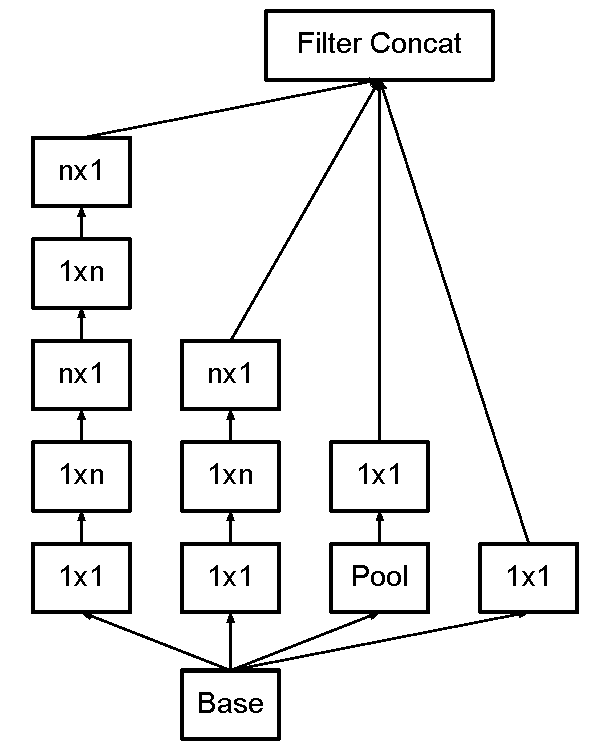
\includegraphics[width=\linewidth]{inceptionv3}
\caption{Inception modules after the factorization of the $n\times n$
convolutions. In our proposed architecture, we chose $n=7$ for the
$17\times 17$ grid. (The filter sizes are picked using principle~\ref{lowdim})}.
\label{fig:inceptionv3}
\end{figure}
\begin{figure}
\centering
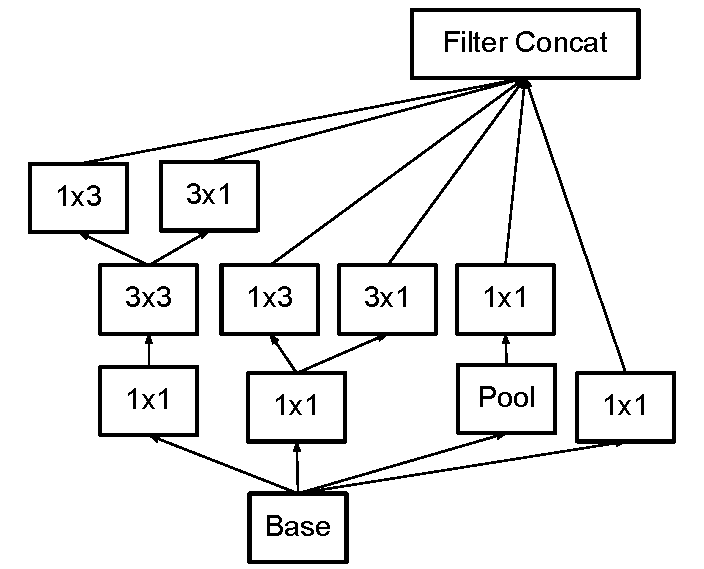
\includegraphics[width=\linewidth]{inceptionv4}
\caption{Inception modules with expanded the filter bank outputs. This
  architecture is used on the coarsest ($8\times 8$) grids to promote
high dimensional representations, as suggested by principle~\ref{highdim} of Section~\ref{principles}.
We are using this solution only on the coarsest grid, since that is the place
where producing high dimensional sparse representation is the most critical
as the ratio of local processing (by $1\times 1$ convolutions) is increased
compared to the spatial aggregation.}
\label{fig:inceptionv4}
\end{figure}

In theory, we could go even further and argue that one can
replace any $n\times n$ convolution by a $1\times n$ convolution followed
by a $n\times 1$ convolution and the computational cost saving increases
dramatically as $n$ grows (see figure 6). In practice, we have found that employing this
factorization does not work well on early layers, but it gives very good results
on medium grid-sizes (On $m\times m$ feature maps, where $m$ ranges between $12$
and $20$). On that level, very good results can be achieved by using
$1\times 7$ convolutions followed by $7\times 1$ convolutions.
